\documentclass[aps,prl,reprint,10pt,amsmath,amssymb,superscriptaddress,a4paper]{revtex4-2}
\usepackage{graphicx} % Graphics package
\usepackage{dcolumn} % Double column package
\usepackage{amsmath,amsfonts,amsthm} % Math packages
\usepackage[margin=2cm]{geometry} % Sets 2cm margins
\usepackage{datetime} % Package for automatic date & time
\usepackage{subfig}
\usepackage[hidelinks]{hyperref}

\begin{document}

\title{Properties of Laser Light (PLL)}

\author{T. Nguyen (z5416116)}
\affiliation{UNSW PHYS3117 - Physics Laboratory}
\date{\currenttime~\today}

\begin{abstract}
l
\end{abstract}

\maketitle

\section{Introduction}

Unfortunately, this is a short report so the lengthy history of the development of the laser cannot be fully treated however the key points will be covered. The theory of lasers 
was well understood way before its invention in 1951 by Charles H. Townes. Although there is heavy dispute around who invented the laser, and even a lawsuit around its patents, the 
first 'laser' was constructed in 1953, using a resonant microwave cavity. Nevertheless, the theory behind stimulated emission was well developed in the early 1920s along with the 
onset of quantum mechanics into the field of physics \citep{hecht}. Using the old quantum theory framework, in a 1917 paper, Einstein theorised the existence of stimulated emission. 
He postulated that photons would prefer to travel together in the same state and therefore, spontaneously emitted photons, for which the name he gave the production of photons from 
electrons dropping down in energy levels, would then lead to or induce other photons to be emitted in the same direction (see Ref \citep{einstein}).

Fast forward a decade, stimulated emission will be experimentally verified in 1928 by Rudolf Walther Ladenburg, who deemed it unpractical and he did not explore the subject any further 
\citep{KopfermannLadenburg1928}. The main subject of this report is the Helium Neon (He-Ne) laser which was invented by Javan, Benenett and Herriott in 1961 \citep{Javan1961}. Surprisely, they did not win 
the Nobel Prize for their invention, rather the 1964 coveted prize went to the aforementioned Townes and his team for their foundational work on the maser and laser. Despite this, the 
He-Ne laser continues to be one of the most influential instruments in the modern development of technology.

The most common use of He-Ne lasers are in the field of optics. They are low cost and have comparatively easier modes of operation than their counter parts, producing beams of similar 
quality in terms of spatial coherence and coherence length \citep{HeliumNeonLaser_Wikipedia_2025}. A simple search on Google scholar for He-Ne laser will reveal a multitude of applications 
across various fields such as physics, biology and medicine.

\section{The He-Ne Laser}

Quantum mechanics states that when an excited electron decays to a lower energy state, it will release a photon with energy equal to the energy difference of the two states. This is called 
spontaneous emission. When the emitted photon travels close to or pass by another excited electron, it may induce the same transition and the photon emitted from this interaction is the result 
of a stimulated emission process. The induced process will produce a photon with the exact same properties as the photon used to stimulate it and therefore, with the correct set up, a laser can 
emit one narrowband range of photons.

For lasers to operate, there must be a population inversion so that the rate of stimulated emission exceeds that of spontaneous emission or absorption. It follows 
that the number of electrons in an excited state will be greater than the number of electrons is a non-excited state. In a He-Ne laser, there is a mixture of neon and helium gas in a tube. The ratio between 
helium and neon atoms is 9:1. There is then an electrical discharge that ionises the gas, causing the helium atoms to enter metastable states. In this state, an electron in the helium atom is excited from 1s 
to 2s level. Because of quantum mechanics selection rules, this state is 'stable', despite it not being the lowest energy state. Therefore, the helium atoms are in a metastable state, where its downward transition 
is forbidden. 

The photons emitted by the laser are generated with collisions between metastable helium atoms and neon atoms. Neon has 10 electrons residing in the 1s, 2s, 2p shells. The collision between a 2p neon electron and a 
metastable helium will excite the neon electron to higher energy states. The most likely state being 4s or 5s, rather than 3s or 3p. Once the collision occurs, the helium electron will fall back down to ground level.
There are, consequently, many different wavelengths of light that can be possibly emitted from a tube of helium and neon gas, as seen in Figure \ref{fig:transitions}

\begin{figure}
    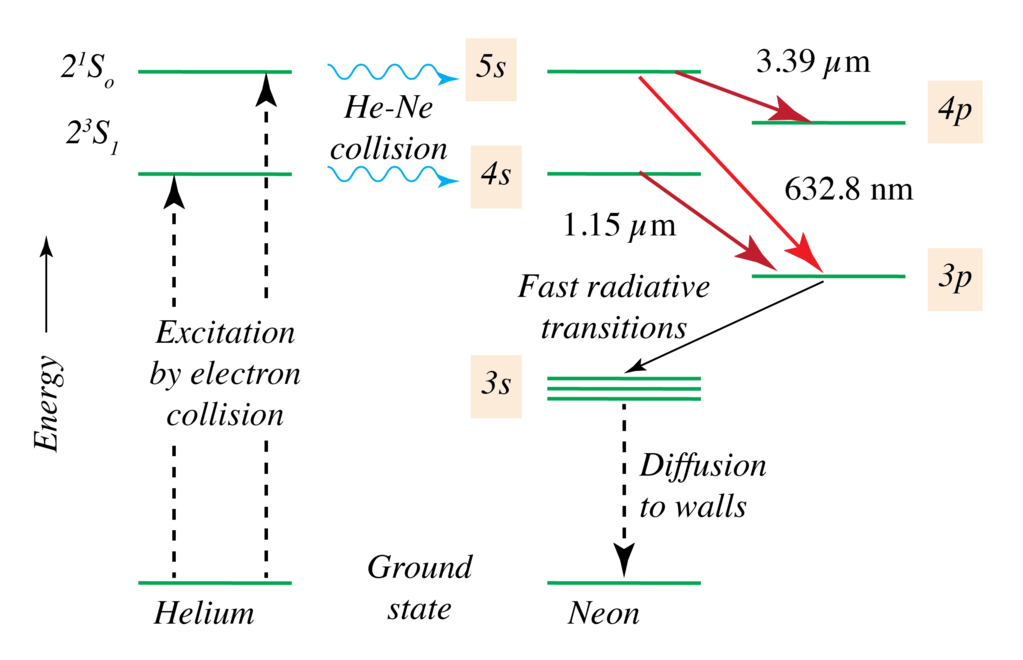
\includegraphics[width=8cm]{../Figures/HeNe_Laser_Levels.png}
    \caption{Possible transitions in the interactions between an excited helium and neon atom. Source: Wikipedia \citep{HeliumNeonLaser_Wikipedia_2025}}.
    \label{fig:transitions}
\end{figure}

\section{Optical cavity}

To select or filter out the desired wavelength, optical cavities are used in lasers. An optical cavity is two mirrors facing each other in a configuration that traps light. In the case of creating an operational laser, 
the light is trapped between a fully and a partially reflecting mirror, seen in Figure \ref{fig:cavity}.

\begin{figure}
    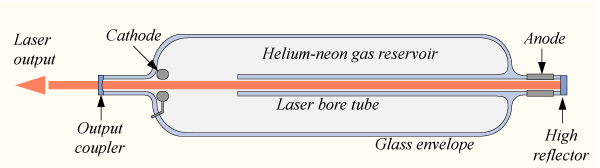
\includegraphics[width=8cm]{../Figures/R1Z7_HeNe-Laser_Tube-Diagram.png}
    \caption{Simple diagram showing the anatomy of the He-Ne laser. The cathode and anode provides the electrical discharge that excites the helium electrons inside the helium-neon gas reservoir that is contained by the glass envelope.
    The output coupler is a partially reflecting mirror of approximately 99\% strength whilst the high reflector is approximately 99.99\%. Therefore the laser output is 1\% of the power of exhibited by the collisions. Source: RPMC lasers 
    \citep{RPMC2025HeNe}}
    \label{fig:cavity}
\end{figure}

\subsection{Longitudinal Modes of Oscillation}

For a standing wave to exist, the path length of the light travelled between mirrors in the optical cavity 
must be an integer number of the wavelengths so $2L = m\lambda$. We can rewrite as a series of resonant frequencies 

\begin{equation}
    \nu = \frac{mc}{2L}.
\end{equation}

The separation of these longitudinal modes is then 

\begin{equation}
    \Delta \nu = \frac{c}{2L}.
\end{equation}

\subsection{Coherence}

Another property that laser lights possess is coherence. Coherence of light can be reduced to the simple fact: given a point in an optical field, $(\textbf{r}_1, t_1)$, can one predict the value of another point in the same optical field 
$(\textbf{r}_2, t_2)$ \citep{reece_coherence_unsw}. Because the spatial and temporal components of the field can be separated, we can analyse the coherence of the light in terms of temporal and spatial coherence.

\subsubsection{Temporal Coherence}

The most simple way to observe temporal coherence is in the Michelson interferometer. If we take a look at Figure \ref{fig:interferometer}, we can find the temporal coherence of light in effect. The visibility of interferometry fringes would oscillate 
but gradually converges as the path difference between the two beams from the same of light increases. In perfectly correlated and in phase waves, the intensity of the fringes would be twice the sum of the individual beams whereas in perfectly uncorrelated 
waves, the intensity of fringes will just be the sum of the two intensities.

\begin{figure}
    
\includegraphics[width=8cm]{../Figures/michelson.png}
    \caption{(a) Schematic diagram of the Michelson interferometer setup. A source of light enters a beam splitter which then directs two beams into a fixed and a movable mirror. The two separate beams then are reflected back into the splitter where 
    they recombine and enter the detector. (b) A graph displaying the intensity of the interferometry pattern based on the path difference, or the difference in distances between the two mirrors.}
    \label{fig:interferometer}
\end{figure}

We can hand wave a derivation for the visibility of fringes using the Wiener-Khinchin theorem which states an autocorrelation (coherence function) is the Fourier transform of the power spectrum. If we take the power spectrum to be a series of Dirac Delta functions 
with a spacing of $\Delta \nu$, where $\nu$ is the longitudinal mode spacing. We will find the magnitude of the coherence function (proportional to the visibility) to have a periodic factor of $\tau_{\text{rev}}=\frac{1}{\Delta \nu}$. Therefore, the coherence length 
can be written in terms of the cavity length,

\begin{equation}
    \Delta_{\text{rev}} = c \tau_{\text{rev}} = \frac{c}{\Delta \nu} = 2L_{\text{cav}}.
\end{equation}

\subsubsection{Spatial Coherence}
Spatial coherence is essentially the measure of coherence in the transverse direction, for two points on the plane of the light's oscillation. This is a simple construction as we can just investigation this coherence by checking the interference pattern 
at these two points using the Young double slit experiment. Using the same result as the temporal coherence, if the two light waves are correlated their intensity sum will be much higher (twice) than the uncorrelated light waves.

\section{Experimental Results \& Analysis}

\subsection{Laser warm up}

\begin{figure*}
    \subfloat[Without polarisation]{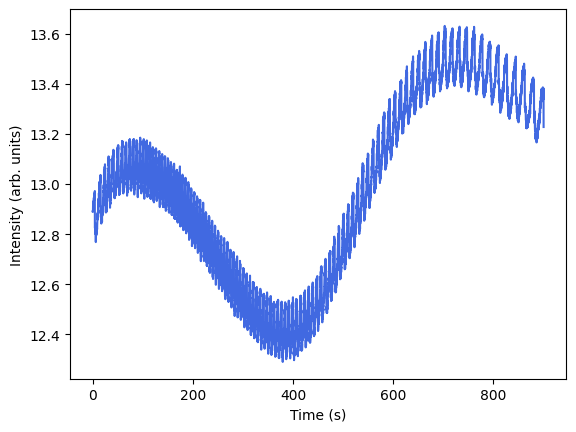
\includegraphics[width=8cm]{../Figures/warmupnopol.png}}
    \subfloat[With polarisation]{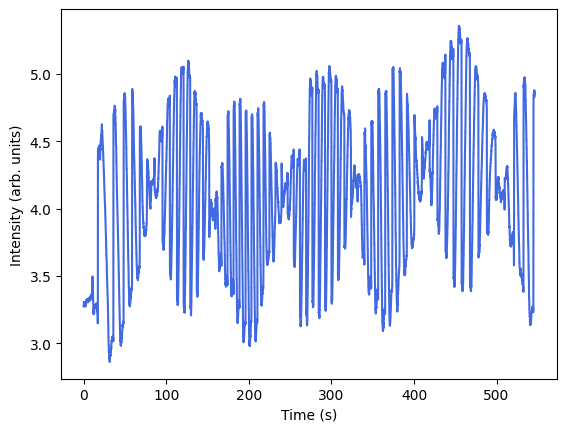
\includegraphics[width=8cm]{../Figures/warmuppol.png}}
    \caption{l}
    \label{fig:warmup}
\end{figure*}

\subsection{Measurement of the wavelength of the laser}

\begin{figure}
    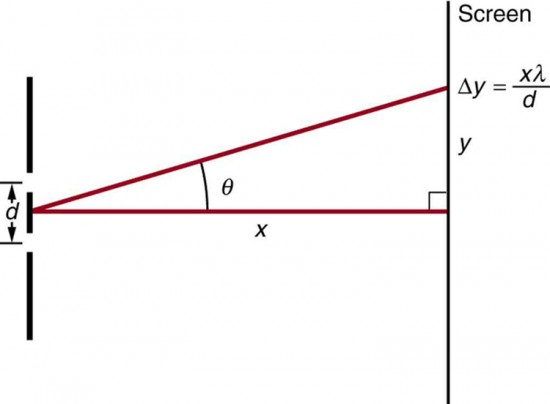
\includegraphics[width=8cm]{../Figures/doubleslit.jpg}
    \caption{l}
    \label{fig:doubleslit}
\end{figure}

\subsection{Longituinal modes}

\subsection{Spatial coherence}

\begin{figure*}
    \centering
    \subfloat{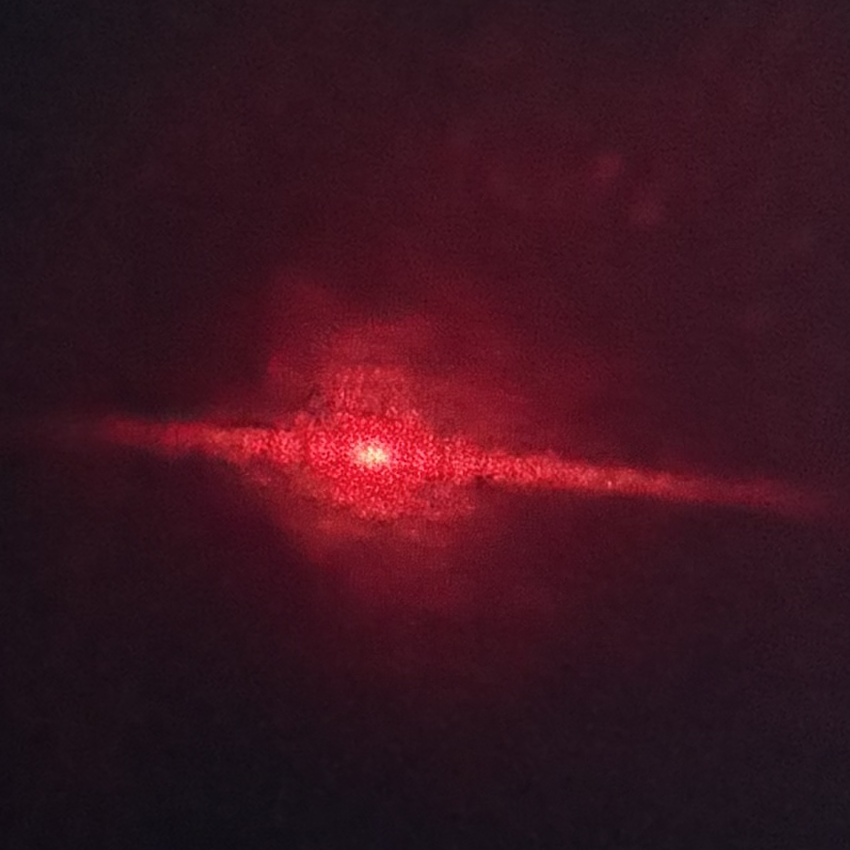
\includegraphics[width=6cm]{../Figures/sc1.png}} \hspace{0.25cm}
    \subfloat{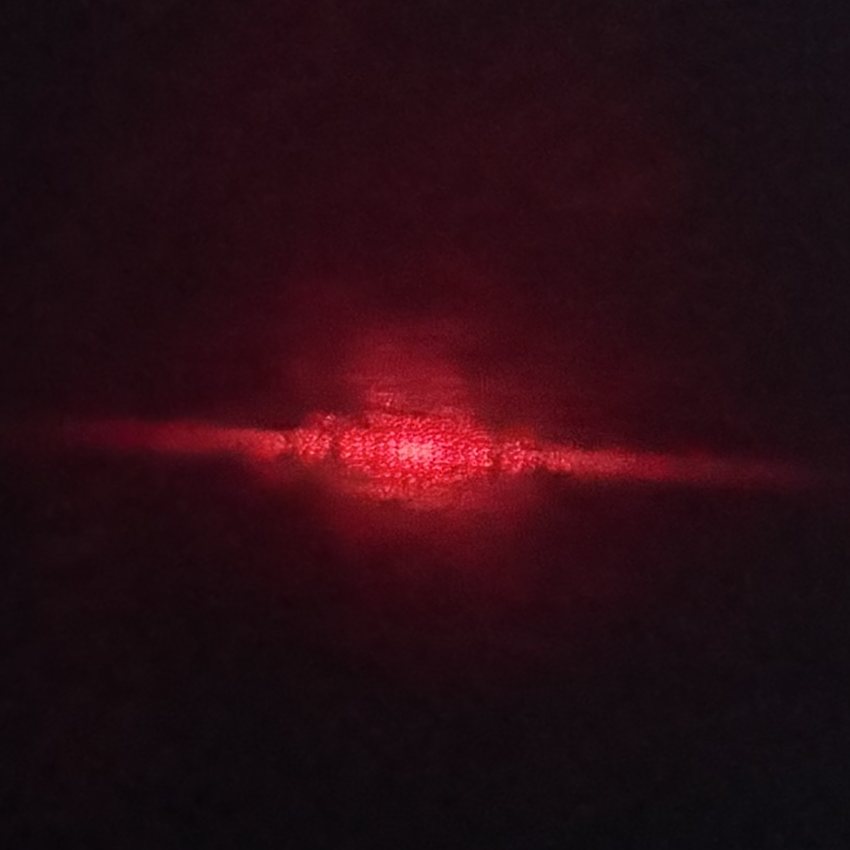
\includegraphics[width=6cm]{../Figures/sc2.png}} \\ \vspace{0.25cm}
    \subfloat{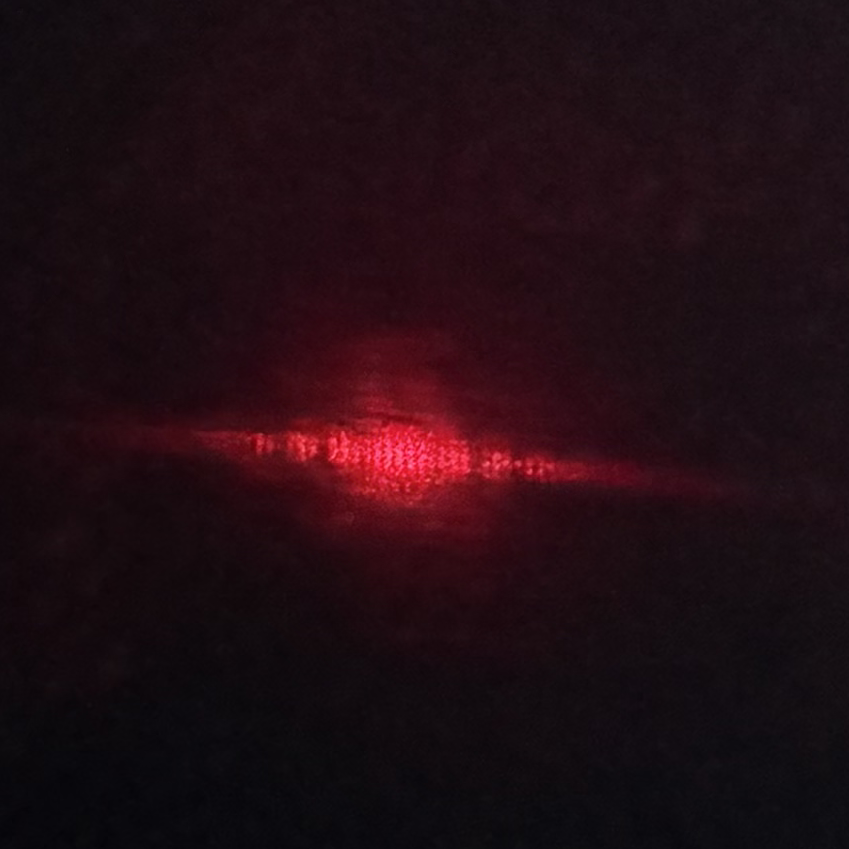
\includegraphics[width=6cm]{../Figures/sc3.png}} \hspace{0.25cm}
    \subfloat{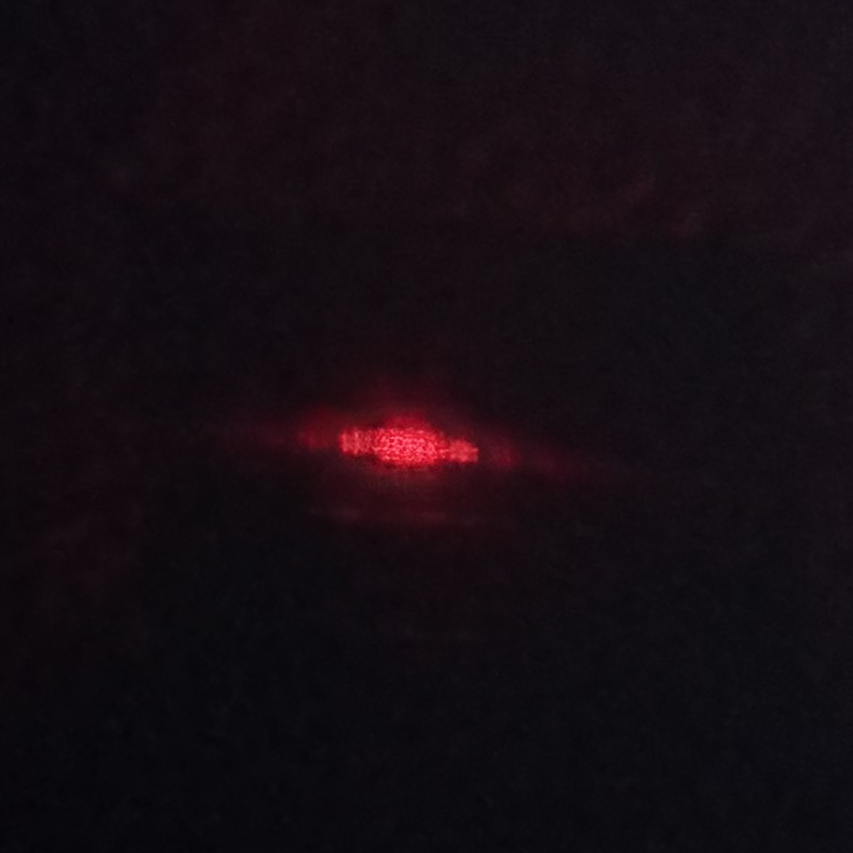
\includegraphics[width=6cm]{../Figures/sc4.png}} \\ \vspace{0.25cm}
    \subfloat{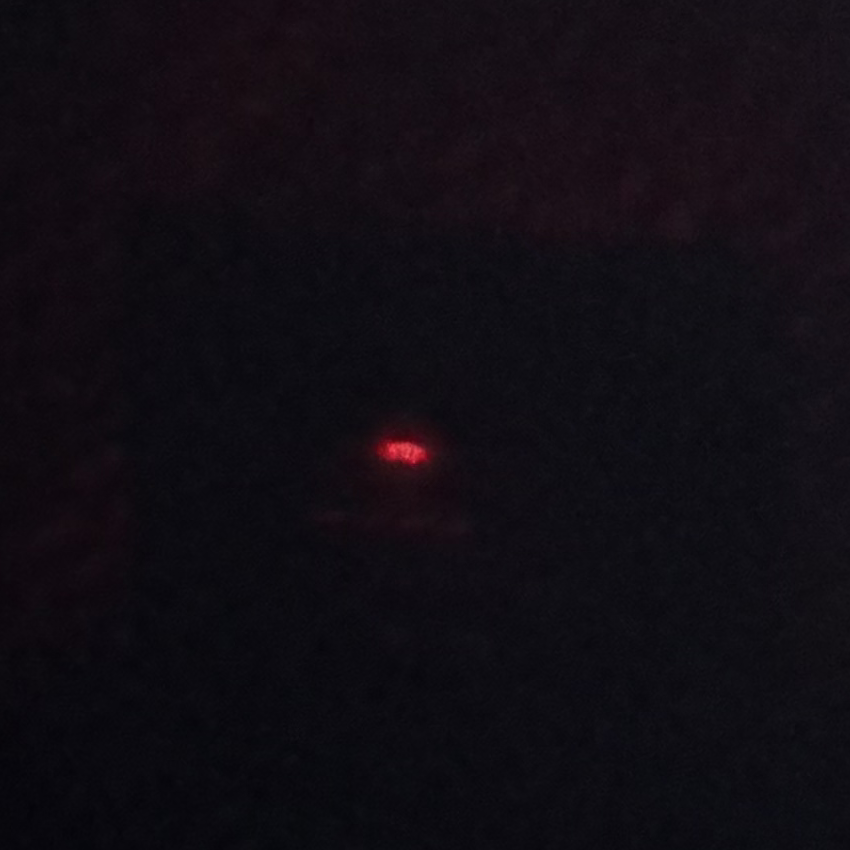
\includegraphics[width=6cm]{../Figures/sc5.png}}
    \caption{l}
    \label{fig:spatialcoherence}
\end{figure*}

\subsection{Temporal Coherence}

\begin{figure}
    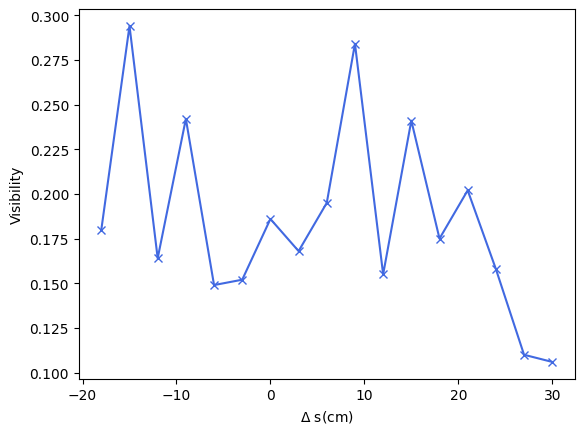
\includegraphics[width=8cm]{../Figures/tempcoherence.png}
    \caption{l}
    \label{fig:temporalcoherence}
\end{figure}

\section{Conclusion}

\section{Acknowledgements}

\bibliographystyle{apsrev4-2}
\bibliography{references}

\end{document}